%% =====================================================================
%%  Confidence-Guided Adaptive Reconstruction for Windowed QPE
%%  Target venue: MethodsX (Elsevier)
%%  Submission draft. Remaining \PLACEHOLDER markers are author-supplied
%%  fields only (affiliation, ORCID, repo URL, DOI, commit, funding).
%%  Build:  pdflatex main / bibtex main / pdflatex x2
%% =====================================================================
\documentclass[preprint,11pt]{elsarticle}

\usepackage{amsmath,amssymb,amsthm}
\usepackage{booktabs}
\usepackage{graphicx}
\usepackage{xcolor}
\usepackage{array}
\usepackage[hidelinks]{hyperref}
\usepackage{tikz}
\usetikzlibrary{arrows.meta,positioning,fit,backgrounds}
\usepackage[section]{placeins}
\usepackage{algorithm}
\usepackage{algpseudocode}

% ---- float placement: without these, the validation tables drift to the
% ---- end of the document, far from the text that discusses them.
\renewcommand{\topfraction}{0.9}
\renewcommand{\bottomfraction}{0.8}
\renewcommand{\textfraction}{0.07}
\renewcommand{\floatpagefraction}{0.7}
\setcounter{topnumber}{3}
\setcounter{bottomnumber}{2}
\setcounter{totalnumber}{5}

% ---- page efficiency (formatting only; no content is affected) -------
\setlength{\bibsep}{2pt plus 0.3ex}
\setlength{\textfloatsep}{10pt plus 2pt minus 2pt}
\setlength{\intextsep}{10pt plus 2pt minus 2pt}
\setlength{\abovedisplayskip}{6pt plus 2pt minus 2pt}
\setlength{\belowdisplayskip}{6pt plus 2pt minus 2pt}

% ---- draft markers: make every open item greppable and visible -------
\newcommand{\TODO}[1]{\textcolor{red}{\textbf{[TODO: #1]}}}
\newcommand{\PLACE}[1]{\textcolor{blue}{\textbf{[PLACEHOLDER: #1]}}}

% ---- evidentiary labels, carried over verbatim from the source notes -
\newcommand{\PROVEN}{\textsc{(proven)}}
\newcommand{\HEUR}{\textsc{(heuristic)}}
\newcommand{\EMPIR}{\textsc{(empirical)}}
\newcommand{\INVAR}{\textsc{(implementation invariant)}}

\newtheorem{proposition}{Proposition}
\newtheorem{lemma}{Lemma}
\newtheorem{corollary}{Corollary}
\newtheorem{invariant}{Invariant}

% Supplementary Information pointers (SI is a separate document, so these
% are literal rather than \ref, which cannot cross documents).
\newcommand{\SI}{Supplementary Information}
\newcommand{\SIproofs}{\SI{}~Sec.~S1}
\newcommand{\SIcalib}{\SI{}~Sec.~S2}
\newcommand{\SIartifacts}{\SI{}~Sec.~S3}

\newcommand{\Cw}{C_w}
\newcommand{\dcov}{\delta_{\mathrm{cov}}}
\newcommand{\Smax}{S_{\max}}
\newcommand{\beammax}{\texttt{beam\_max}}

\journal{MethodsX}

\begin{document}

\begin{frontmatter}

\title{Confidence-Guided Adaptive Reconstruction for Windowed Quantum
Phase Estimation}
% Optional subtitle, if you want one --- uncomment and merge into \title:
% A drop-in classical post-processing replacement for fixed-budget
% candidate reconstruction in modular Shor

\author[inst1]{Sanjay Lakshmanan R}
\ead{rajasanjay21@gmail.com}

\address[inst1]{Department of Computer Science and Engineering,
Amrita Vishwa Vidyapeetham, Chennai, India}

\begin{abstract}
Windowed quantum phase estimation replaces one wide phase register with
several narrow, independently measured windows and reassembles a
full-precision phase classically. The published reconstruction stage gives
every window a fixed budget --- constant retained candidates, constant beam
width, constant shots --- however decisive that window's measurement was.

We describe confidence-guided adaptive reconstruction, a drop-in
customisation of the classical stage that leaves the quantum circuit, its
width, its depth and its sampling procedure unchanged. A per-window
posterior comparison statistic $\Cw$, computed from counts already
measured, drives three independently switchable modules: coverage-based
candidate retention, ambiguity-scaled beam width, and confidence-gated shot
stopping. With all three disabled the implementation reduces to the
published pipeline, verified trial by trial.

Validation is at the window level, against exact noiseless marginals from
statevector simulation. Over 3{,}354 windows, coverage-based retention
raises retained true probability mass from $0.571$ to $0.841$. The gain is
not superiority over a well-chosen fixed budget --- at $k=16$ it is
marginally worse --- but insensitivity to the choice: it holds near $0.98$
across $k$, where fixed retention ranges $0.29$ to $1.00$.

$\Cw$ is a modest ranking signal (AUC $0.640$) and measurably overconfident
(Brier $0.2239$), so it must not be read as a calibrated probability.
End-to-end factorisation evidence, and matched-resource controls showing
that no individual module beats an equally-resourced uniform allocation,
are reported in the companion study~\cite{companion}.
\end{abstract}

\begin{keyword}
Quantum phase estimation \sep Shor's algorithm \sep classical
post-processing \sep adaptive resource allocation \sep Bayesian posterior
comparison \sep beam search
\end{keyword}

\end{frontmatter}

% =====================================================================
\section*{Highlights}
\begin{itemize}\itemsep2pt
\item A per-window Bayesian statistic sets candidate, beam and shot budgets
      from the already-measured counts; the quantum circuit is unchanged.
\item Coverage-based retention captures $0.841$ of true per-window
      probability mass against $0.571$ for a fixed budget, over 3{,}354
      windows.
\item Its value is insensitivity to the budget setting, not superiority at
      any one setting.
\item $\Cw$ ranks windows usefully at module D's operating point but is not
      a calibrated probability.
\end{itemize}

% =====================================================================
\section*{Specifications table}

\begin{center}
\small
\begin{tabular}{@{}p{0.30\linewidth}p{0.64\linewidth}@{}}
\toprule
\textbf{Subject area} & Physics and Astronomy \\
\midrule
\textbf{More specific subject area} & Quantum computing; quantum
algorithms; classical post-processing for quantum phase estimation \\
\midrule
\textbf{Name of your method} & Confidence-Guided Adaptive Reconstruction
for Windowed Quantum Phase Estimation \\
\midrule
\textbf{Name and reference of original method} & Windowed quantum phase
estimation with carry-aware candidate stitching, as specified by Shukla
and Vedula \cite{wqpe2025,modularshor2025} (Algorithm 3 of the latter). \\
\midrule
\textbf{Resource availability} & Code, experiment scripts and all raw
result data: \url{https://github.com/Shadow-46/QuantumPhaseReconstruction} (Apache-2.0). An
archived snapshot will be deposited in a persistent repository and its
DOI supplied at acceptance. Dependencies: Python 3.12,
Qiskit \cite{qiskit2024} 2.4.1, Aer 0.17.2, SciPy 1.17.1, NumPy 2.4.6,
scikit-learn 1.9.0. No quantum hardware required.
Script-to-artifact map: \SIartifacts{}. Versions are pinned to those
that produced the released results. \\
\bottomrule
\end{tabular}
\end{center}

\noindent
\textit{Note on scope.} This article customises only the \emph{classical
reconstruction} stage of the original method. No change is made to the
quantum circuit, its qubit count, its depth, or its sampling procedure.
The method is therefore reusable by any implementation of windowed phase
estimation that produces per-window measurement counts, independently of
how those counts were generated.

% =====================================================================

% =====================================================================
\section*{Graphical abstract}

\noindent
A landscape rendering of Figure~\ref{fig:schematic}, with the three
adaptive modules annotated by the fixed quantity each replaces
($k\to m_w$, $P\to P'$, $S_w\to$ resampled $S_w$), and a caption strip
carrying the window-level comparison: fixed-budget retention captures
$0.571$ of true probability mass, coverage-based retention $0.841$.
Supplied as a separate image file at submission.

% =====================================================================
\section*{Introduction}
\label{sec:intro}

Shor's algorithm \cite{shor1997} reduces integer factorisation to
order-finding, and order-finding to quantum phase estimation
\cite{kitaev1995,cleve1998,nielsenchuang}. Textbook QPE requires a phase
register as wide as the requested precision, which is exactly the resource
near-term hardware does not have. The windowed formulation
\cite{wqpe2025,modularshor2025} removes that requirement by partitioning
the register into narrow, independently measured, overlapping windows and
reassembling the phase classically. The quantum saving is real, and it is
bought with classical work: reconstruction must now recover one phase from
$W$ partial, individually ambiguous measurements.

That classical stage is where this article intervenes. Three of its
quantities are compile-time constants in the published method --- how many
candidate patterns to retain per window, how wide a beam to carry through
stitching, and how many shots to spend per window --- and they are
identical for every window of every instance, however decisive that
window's measurement turned out to be. A prior characterisation of our own
reproduction attributed 72\% of its observed failures to this uniform
allocation rather than to noise or to any defect in the reconstruction
logic. That campaign is reported in the companion
study~\cite{companion}; here it is the design brief.

The customisation replaces each constant with a quantity computed from
counts already measured, via a per-window posterior comparison statistic.
It changes no circuit, adds no qubit, and reduces exactly to the published
pipeline when switched off --- a property of the implementation we verified
rather than assumed.

One scoping note shapes everything that follows. These modules do not
outperform a well-chosen fixed budget: against a control handed the same
realised budget to spend uniformly, no individual module is
distinguishable from it. What they remove is the need to choose that budget
correctly in advance. The defensible contribution is automatic budget
selection, not superior placement.

\paragraph{Contributions.} (i) A per-window posterior comparison statistic
$\Cw$, an exact two-proportion Bayesian comparison over the top-two
observed patterns, with proven ordinal properties (Sec.~\ref{sec:cw}).
(ii) Three independently switchable modules driven by the sampled counts,
with a verified equivalence to the published baseline when all are disabled
(Algorithm~\ref{alg:adaptive}, Invariant~\ref{prop:baseline}) --- what makes
the method safe to adopt incrementally. (iii) A reusable adoption protocol
(Sec.~\ref{sec:protocol}) and a cost analysis separating classical
asymptotics from module D's additional \emph{quantum} sampling
(Sec.~\ref{sec:cost}). (iv) Window-level validation against exact noiseless
marginals (Sec.~\ref{sec:validation}): over 3{,}354 windows, coverage-based
retention captures $0.841$ of the true probability mass against $0.571$ for
a fixed budget, almost independently of how that budget was set. (v) A
calibration study (Sec.~\ref{sec:calibration}) showing $\Cw$ ranks usefully
where module D consults it, while being a poor probability estimate
overall.
\section{Method details}

\subsection{The original method and the three constants it fixes}
\label{sec:baseline}

Quantum phase estimation recovers an eigenphase $\varphi$ of a unitary
$U$ from measurements of a phase register \cite{kitaev1995,cleve1998}.
In Shor's order-finding reduction \cite{shor1997}, $U_a\lvert
y\rangle=\lvert ay \bmod N\rangle$ has eigenphases $s/r$ for the
multiplicative order $r=\mathrm{ord}_N(a)$; continued-fraction expansion
of a measured phase recovers $r$, and factors follow from
$\gcd(a^{r/2}\pm1,N)$ \cite{nielsenchuang}.

Standard QPE requires a phase register as wide as the requested
precision, which is prohibitive on shallow hardware. The windowed
formulation \cite{wqpe2025,modularshor2025} instead partitions the
$\ell$-bit phase interval into $W$ overlapping windows. Window $w$
covers bit positions $[\mathrm{start}_w,\mathrm{start}_w+\mathrm{width}_w)$
with $\mathrm{start}_{w+1}=\mathrm{start}_w+\mathrm{width}_w-o$ for
overlap $o$, and is measured by its own circuit allocating only
$\mathrm{width}_w$ phase qubits --- never $\ell$. Circuit width is thus
decoupled from total precision, which is the formulation's central
resource claim.

The cost of that decoupling is borne entirely by the classical stage,
which must reassemble one full-precision phase from $W$ partial and
possibly ambiguous local measurements. Given per-window count
dictionaries $\mathrm{counts}_w:\{0,1\}^{\mathrm{width}_w}\to
\mathbb{Z}_{\geq0}$ with $S_w=\sum_b \mathrm{counts}_w(b)$ shots, the
published pipeline proceeds in three steps:

\begin{enumerate}\itemsep1pt
\item \textbf{Candidate generation.} Rank each window's observed patterns
by empirical probability $\hat p_w(b)=\mathrm{counts}_w(b)/S_w$ and
retain the top $k$ (\texttt{candidate\_count}), each encoded at its
absolute bit position.
\item \textbf{Carry-aware beam stitching.} Extend paths across adjacent
windows, admitting a pair when its overlapping bits agree exactly or
after one legitimate single-bit borrow; score paths by the product of
candidate probabilities and retain the top $P$ (\texttt{max\_paths}) at
each level.
\item \textbf{Order recovery.} Apply continued-fraction expansion to each
stitched phase in ranked order until one yields a non-trivial
factorisation.
\end{enumerate}

Three quantities are fixed constants here, chosen at configuration time
and identical for every window of every instance: the candidate count
$k$, the beam width $P$, and the per-window shot count $S_w$. Our method
replaces all three with data-dependent quantities computed from the
already-sampled counts, as shown schematically in
Figure~\ref{fig:schematic}. A symbol table is given in \SIproofs{};
every symbol is also defined where it first appears below.

\begin{figure}[htbp]
\centering
\resizebox{\linewidth}{!}{%
\begin{tikzpicture}[
  font=\small,
  box/.style={draw, rounded corners, align=center, minimum height=1.05cm, minimum width=2.05cm, inner sep=3pt},
  mod/.style={draw, dashed, rounded corners, align=center, minimum height=0.85cm, fill=gray!8, inner sep=3pt},
  arr/.style={-{Latex[length=2.2mm]}, thick},
  node distance=6mm
]

\node[box] (sample) {Windowed\\quantum sampling\\[1pt]\footnotesize $W$ shallow\\circuits, widths\\$\mathrm{width}_1,\dots,\mathrm{width}_W$};
\node[box, right=of sample] (counts) {Per-window\\counts $\mathrm{counts}_w$\\[1pt]\footnotesize $S_w$ shots each};
\node[box, right=of counts] (candgen) {Candidate\\generation};
\node[box, right=of candgen] (stitch) {Carry-aware\\beam stitching};
\node[box, right=of stitch] (order) {Continued-fraction\\order recovery};
\node[box, right=of order] (factors) {Factors of $N$};

\draw[arr] (sample) -- (counts);
\draw[arr] (counts) -- (candgen);
\draw[arr] (candgen) -- (stitch);
\draw[arr] (stitch) -- (order);
\draw[arr] (order) -- (factors);

\node[mod, below=9mm of counts] (moduleD) {Module D: $\Cw$ per window;\\below threshold $\Rightarrow$ more shots\\(cap $\Smax$)};
\node[mod, below=9mm of candgen] (moduleB) {Module B: retain\\candidates to coverage\\$\dcov$ (adaptive $m_w$)};
\node[mod, below=9mm of stitch] (moduleC) {Module C: beam width\\$P'$ scales with\\coverage-expansion rate\\(cap $\beammax$)};

\draw[arr] (moduleD) -- (counts);
\draw[arr, dashed] (moduleD.north) -- ++(0,3mm) -| (sample.south);
\draw[arr] (moduleB) -- (candgen);
\draw[arr] (moduleC) -- (stitch);

\end{tikzpicture}%
}
\caption{Method schematic. The published pipeline (top row, solid) samples
each window once at a fixed shot budget, retains a fixed candidate count,
and stitches with a fixed beam width. The three adaptive modules
(dashed, bottom) replace each fixed budget with a quantity computed from
the already-sampled counts: module D re-samples ambiguous windows before
candidate generation proceeds (dashed feedback arrow into the sampling
stage), module B expands candidate retention to a target probability
mass, and module C widens the beam in proportion to how often module B
needed to expand coverage. All three modules are independently
switchable and the pipeline reduces to the published baseline when all
three are disabled.}
\label{fig:schematic}
\end{figure}



\subsection{Motivating evidence: fixed budgets are the binding constraint}
\label{sec:motivation}

The method was not designed from intuition. It was designed against a prior
black-box failure-mode characterisation of our own reproduction of the
published pipeline, reported in full in the companion
study~\cite{companion}. Two findings from it define the design target and
are the only ones this article depends on. Varying any single parameter in
isolation produced no failures across 435 one-factor-at-a-time trials,
whereas starving several budgets together failed 47.9\% of the time on an
instance the same pipeline solves trivially when any one budget is relaxed.
Replaying every observed failure through a fixed counterfactual ladder
attributed 72\% of them to classical budget starvation rather than to
noise, corruption, or any defect in the reconstruction logic.

That attribution is what selects the classical reconstruction stage, rather
than the circuit or the noise model, as the place to intervene: the
failures are caused by spending a fixed classical budget on windows that
needed an unequal one.

\subsection{Relation to existing adaptive and Bayesian approaches}
\label{sec:related}

Adaptivity and Bayesian inference are both well established in quantum
estimation, so it is worth being precise about what is and is not new
here.

\emph{Bayesian amplitude- and phase-estimation methods}
\cite{bae2025,biqae2026,vqae2022} maintain a posterior over the estimated
quantity and use it to choose the next \emph{quantum} query --- which
circuit to run, at what depth, for how many shots --- to reduce quantum
query complexity. Module D is a deliberately narrower relative of that
idea. The difference is what the posterior governs: those methods
optimise the quantum sampling schedule, whereas modules B and C spend no
quantum resources at all and reallocate a purely classical budget over
counts already measured. The two are complementary, and nothing prevents
combining them.

\emph{Existing windowed-reconstruction pipelines}
\cite{wqpe2025,modularshor2025} already contain multi-candidate
retention, carry-aware stitching and beam-search pruning; we reproduce
all three unchanged. What they lack is any rule connecting the budget a
window receives to how ambiguous that window's measurement was: overlap
is static, and the candidate count and beam width are constants.

\emph{Exhaustive reconstruction} --- searching every consistent path
rather than a bounded beam --- is the exactness endpoint of the same axis,
at a cost combinatorial in the number of windows. Our framework
approaches it in the joint limit $\Smax\to\infty$, $\dcov\to0$,
$\beammax\to\infty$, so the relationship is one of degree rather than
kind. We make no claim about specific published exhaustive or
dynamic-programming algorithms, having surveyed the class rather than
benchmarked a named implementation.

Table~\ref{tab:novelty} places the present work against these lines
along the dimensions that distinguish them. The reproduced components
occupy the same cells as the source method by construction; the two
rightmost columns are where this article differs, and the adaptive-sampling
cell differs only in the restricted sense its footnote records.

\begin{table}[htbp]
\centering\footnotesize
\caption{Positioning against the cited prior work.
\checkmark~= present and adaptive; \emph{fixed} = present but set at
configuration time; ---~= not applicable to that method. Reproduced
components ($\ast$) occupy the same cells as the source method by
construction; the two rightmost columns are where this article differs. The
table compares only works cited here, and only on dimensions those works
address; it is not a survey.}
\label{tab:novelty}
\setlength{\tabcolsep}{3.2pt}
\begin{tabular}{@{}p{0.215\linewidth}cccccc@{}}
\toprule
 & \shortstack{Windowed\\circuits}
 & \shortstack{Multi-\\candidate}
 & \shortstack{Carry-aware\\stitching}
 & \shortstack{Bounded\\beam}
 & \shortstack{Adaptive\\sampling}
 & \shortstack{\textbf{Adaptive}\\\textbf{cl. budget}} \\
\midrule
Standard QPE \cite{kitaev1995,cleve1998}
  & ---        & ---            & ---        & ---            & ---        & --- \\[2pt]
Windowed / modular WQPE \cite{wqpe2025,modularshor2025}
  & \checkmark & \emph{fixed}   & \checkmark & \emph{fixed}   & ---        & --- \\[2pt]
Bayesian amplitude / phase estimation \cite{bae2025,biqae2026,vqae2022}
  & ---        & ---            & ---        & ---            & \checkmark & --- \\[2pt]
\textbf{This work}
  & \checkmark$^{\ast}$ & \checkmark & \checkmark$^{\ast}$ & \checkmark
  & \checkmark$^{\dagger}$ & \checkmark \\
\bottomrule
\end{tabular}

\vspace{3pt}
\begin{minipage}{\linewidth}\footnotesize
$\ast$~Reproduced unchanged from the source method, not a contribution of
this article. \quad
$\dagger$~Module D adapts only \emph{how many shots} an already-specified
window circuit receives; it never changes which circuit is run, unlike
the Bayesian methods in row 3.
\end{minipage}
\end{table}

The gap we address is therefore specific: \emph{a rule that sets the
classical reconstruction budget --- candidates retained, beam width, and
shots per window --- from the measured counts, leaving the quantum
circuit and its resource profile untouched}. We have not found this
combination proposed for windowed phase estimation, and our survey
covered Bayesian, maximum-likelihood, machine-learning,
dynamic-programming, beam-search and graph-search reconstruction. We
state that as the outcome of a survey rather than as an absence proof.

Two qualifications belong here rather than in a later section: the
statistic is confidence-\emph{driven}, not confidence-\emph{calibrated}
(Sec.~\ref{sec:calibration}), and what it contributes at the scales we
can reach is the automatic selection of a budget, not a superior
placement of one~\cite{companion}. A reader comparing against a
well-tuned fixed budget should expect parity; the value on offer is that
no tuning is needed to reach it.

\subsection{The posterior comparison statistic $\Cw$}
\label{sec:cw}

The one new piece of mathematics the framework depends on is a per-window
statistic that is aware of how much evidence a window's ranking actually
rests on. Let $b^{(1)}_w$ and $b^{(2)}_w$ be the two most-observed bit
patterns in window $w$, with counts $n_1 \ge n_2$ out of $S_w$ shots.
Model each pattern's marginal success count as Binomial and place an
independent Jeffreys prior $\mathrm{Beta}(\tfrac12,\tfrac12)$
\cite{jeffreys1946} on each marginal probability, giving posteriors
$X_i\sim\mathrm{Beta}(\alpha_0+n_i,\ \alpha_0+S_w-n_i)$, $i\in\{1,2\}$,
$\alpha_0=\tfrac12$. Define

\begin{equation}
\Cw \;\mathrel{:=}\; \Pr\!\big[X_1 > X_2\big]
\;=\; \int_0^1 f_{X_1}(x)\,F_{X_2}(x)\,\mathrm{d}x ,
\label{eq:cw}
\end{equation}

with $f_{X_1}$ the density of $X_1$ and $F_{X_2}$ the distribution
function of $X_2$. Equation~\eqref{eq:cw} is evaluated directly, so
$\Cw$ is exactly the stated posterior quantity up to quadrature
tolerance.

\paragraph{What $\Cw$ is, stated precisely.} Under the sampling model
(A1) \emph{and} the working independence assumption (A2) of
Sec.~\ref{sec:assumptions}, $\Cw$ is the posterior probability that
$p_w(b^{(1)}_w) > p_w(b^{(2)}_w)$. Assumption (A2) is false --- the two
counts are negatively correlated coordinates of one $K_w$-way multinomial,
so the exact posterior is a Dirichlet marginal comparison, not a
comparison of two independent Beta variables --- and the size of the
resulting error is measured in Sec.~\ref{sec:calibration}. We therefore
use the term \textbf{posterior comparison statistic} throughout, and we
do \emph{not} describe $\Cw$ as a calibrated probability, a confidence
level with guaranteed coverage, or an error rate. Its established
properties are ordinal (Table~\ref{tab:properties}); its role in the
method is to \emph{rank}
windows by how thin their evidence is, and every use downstream depends
only on that ranking together with one threshold whose value is a tuning
parameter rather than a guarantee.

\paragraph{Why this statistic and not a simpler one.}
Raw probability, top-1/top-2 margin, and entropy over the observed counts
are all \emph{sample-size-blind}. A $2/4$ split and a $500/1000$ split
score identically under every one of them, even though the first is
nearly uninformative and the second nearly certain. Since the dominant
measured failure mode is under-sampling rather than genuine ambiguity
(Sec.~\ref{sec:motivation}), a statistic that cannot tell these apart is
the wrong instrument. Equation~\eqref{eq:cw} is the minimal quantity that
separates them from a single closed definition. A likelihood-ratio test
between ``$b^{(1)}$ true'' and ``$b^{(2)}$ true'' behaves almost
identically --- both reduce to a function of the margin over its standard
error --- so nothing is gained by preferring it, and the posterior form
states more transparently what is being computed. We claim only that
$\Cw$ separates the two regimes with a single unconditional formula, not
that it is optimal among statistics that could do so.

\paragraph{Numerical evaluation.} For general real shape parameters,
$\Pr[X_1>X_2]$ between independent Beta variables has no elementary
closed form. A finite closed-form sum exists when one shape parameter is
a positive \emph{integer}, but here $b_i=0.5+(S_w-n_i)$ is always a
half-integer, so that identity does not apply without separate
derivation. We therefore evaluate Eq.~\eqref{eq:cw} directly by adaptive
quadrature, exact up to floating-point and solver tolerance and requiring
no case-specific formula. This gives a single unconditional code path: no
normal approximation, no Monte Carlo, no branching by shot count or
regime. We do not claim a closed form is unobtainable for half-integer
parameters --- only that the method does not need one.

\subsection{Module B --- coverage-based candidate retention}
\label{sec:moduleB}

Replace the fixed truncation at $k$ with a coverage rule. Rank patterns
by $\hat p_w$ descending and return the \emph{shortest} prefix whose
cumulative empirical mass reaches a target:

\begin{equation}
m_w \;=\; \min\Big\{\, m \ge 1 \;:\; \sum_{i=1}^{m}\hat p_w(b_{(i)}) \;\ge\; 1-\dcov \,\Big\}.
\label{eq:moduleB}
\end{equation}

A near-deterministic window collapses to $m_w=1$, strictly cheaper than
the baseline's $k\ge2$; a genuinely ambiguous one expands as far as the
observed distribution requires. No posterior smoothing is applied before
ranking: at the shot counts tested, Jeffreys smoothing shifts any single
probability by at most $\alpha_0/(\alpha_0 2^{\ell_w}+S_w)\approx0.015$
(the smoothing bound, Table~\ref{tab:properties}), which does not
change the ranking.

\subsection{Module C --- ambiguity-scaled beam width}
\label{sec:moduleC}

Count how many windows the \emph{baseline} truncation would have
under-covered, then widen the beam proportionally:

\begin{align}
\mathrm{expanded} &= \#\Big\{\, w : \sum_{i=1}^{k}\hat p_w(b_{(i)}) < 1-\dcov \,\Big\},
\label{eq:expanded}\\[2pt]
P' &= \min\!\big(\beammax,\; P\cdot(1+\mathrm{expanded})\big).
\label{eq:moduleC}
\end{align}

Note that $\mathrm{expanded}$ is computed against the fixed baseline $k$,
\emph{independently} of whether module B is enabled. This is deliberate:
it is what keeps B and C separately switchable arms of the same ablation
rather than confounded with one another.

\emph{Evidential status.} Of the three modules, C is the one our data
support least. Its independent effect is small on the design grid, absent
on two of three held-out instances, does not survive multiple-comparison
correction, and is indistinguishable from a beam-matched control on every
trial~\cite{companion}. We retain it in the
framework as a combinatorial safeguard --- it provably never narrows the
beam (Table~\ref{tab:properties}), and the attribution analysis of
Sec.~\ref{sec:motivation} identified 20 failures needing candidate budget
and beam width relaxed \emph{together} --- but we do not present it as
independently validated, and Sec.~\ref{sec:protocol} recommends against
enabling it alone.

\subsection{Module D --- confidence-gated shot stopping}
\label{sec:moduleD}

For each window, evaluate $\Cw$ on the current counts. If
$\Cw \ge 1-\varepsilon$, stop. Otherwise draw
$\min(S_w,\ \Smax-S_w)$ further shots from the same operator and
eigenstate, merge the counts, and repeat until either the threshold is
met or the cap $\Smax$ is reached. Shots are thus spent only on the
windows whose evidence is actually thin. This directly targets the 48 of
69 combined-stress failures that the attribution ladder resolved by
additional shots alone.

Module D is the only module that returns to the quantum sampler, and it
is correspondingly the most expensive: each round is one real transpile
and run, measured at ${\approx}3.3$\,s in our environment, which makes it
the dominant wall-clock cost of the framework whenever it triggers
(Sec.~\ref{sec:cost}).

\subsection{The complete adaptive reconstruction procedure}
\label{sec:algorithm}

Algorithm~\ref{alg:adaptive} states the three modules in the order the
implementation applies them. The three boolean flags are what make the
arms of Sec.~\ref{sec:validation} arms of one procedure rather than
separate pipelines: setting all three to \textsc{false} yields exactly
the published baseline (Invariant~\ref{prop:baseline}).

\begin{algorithm}[htbp]
\caption{Confidence-guided adaptive reconstruction. Inputs are the
window specifications, the sampling configuration, the three module
flags, and the parameters of Table~\ref{tab:params}. Lines marked
\textbf{[D]}, \textbf{[B]} and \textbf{[C]} are the only departures from
the published pipeline.}
\label{alg:adaptive}
\small
\begin{algorithmic}[1]
\Require window specs $\{\mathrm{spec}_w\}_{w=1}^{W}$; shots $S^{(0)}$;
flags $\textit{useD},\textit{useB},\textit{useC}$; $\dcov,\varepsilon,\Smax,\beammax$; fixed $k,P$
\Ensure factors of $N$, or \textsc{fail}
\State $\mathrm{counts}_w \gets \textsc{Sample}(\mathrm{spec}_w, S^{(0)})$ for all $w$
\Statex
\If{\textit{useD}}\Comment{\textbf{[D]} confidence-gated shot stopping}
  \For{$w = 1$ \textbf{to} $W$}
    \While{$\Cw(\mathrm{counts}_w) < 1-\varepsilon$}
      \State $\Delta \gets \min(S_w,\ \Smax - S_w)$
      \State \textbf{if} $\Delta \le 0$ \textbf{then break}
        \Comment{cap reached; terminates by Table~\ref{tab:properties}}
      \State $\mathrm{counts}_w \gets \mathrm{counts}_w \uplus \textsc{Sample}(\mathrm{spec}_w, \Delta)$
    \EndWhile
  \EndFor
\EndIf
\Statex
\For{$w = 1$ \textbf{to} $W$}\Comment{candidate generation}
  \If{\textit{useB}}\Comment{\textbf{[B]} coverage-based retention}
    \State $G_w \gets$ shortest prefix of $\mathrm{counts}_w$ ranked by
           $\hat p_w$ with mass $\ge 1-\dcov$ \Comment{Eq.~\eqref{eq:moduleB}}
  \Else
    \State $G_w \gets$ top-$k$ patterns of $\mathrm{counts}_w$ by $\hat p_w$
  \EndIf
\EndFor
\Statex
\If{\textit{useC}}\Comment{\textbf{[C]} ambiguity-scaled beam width}
  \State $e \gets \#\{w : \text{top-}k\text{ mass of } \mathrm{counts}_w < 1-\dcov\}$
         \Comment{Eq.~\eqref{eq:expanded}; uses fixed $k$, not $m_w$}
  \State $P' \gets \min(\beammax,\ P\,(1+e))$
\Else
  \State $P' \gets P$
\EndIf
\Statex
\State $\Phi \gets \textsc{CarryAwareBeamStitch}(G_1,\dots,G_W;\ P')$
       \Comment{unchanged from baseline}
\For{$\hat\phi \in \Phi$ in descending score order}
  \State $f \gets \textsc{RecoverOrderAndFactors}(\hat\phi, a, N)$
         \Comment{unchanged from baseline}
  \State \textbf{if} $f \ne \varnothing$ \textbf{then return} $f$
\EndFor
\State \Return \textsc{fail}
\end{algorithmic}
\end{algorithm}

\subsection{A retracted module and an unchanged carry check}
\label{sec:retraction}

The original design specified a fourth module, A, to fix an apparent defect
in the carry-aware overlap check, on the strength of our own earlier audit
reporting a 55.4\% false-accept rate. Re-validating that evidence before
writing any code showed the finding was wrong, and wrong in the audit
rather than in the mechanism; the companion study~\cite{companion} gives
the defect, the corrected counts, and the three independent checks that
establish the correction. Lemma~\ref{lem:carry} states the algebraic half
of it: the implementation's acceptance condition and the audit's
ground-truth oracle reduce to the same Boolean function, so the original
test could only ever have detected its own bug.

Two consequences follow for this article. Module A was removed from the
design before any code was written, and the carry-check implementation
required no change --- it is inherited from the original method untouched,
and none of the three modules described below acts on it.

\subsection{Assumptions and parameters}
\label{sec:assumptions}

Every property in Sec.~\ref{sec:properties} is conditional on the
following five assumptions. We state them explicitly because one is
measurably false and is retained anyway as a documented scope decision.

\begin{description}\itemsep2pt
\item[(A1) Per-window multinomial sampling.]
Each window's counts are distributed as
$\mathrm{Multinomial}(S_w,\,p_w(\cdot))$, independently across windows.
This is the standard model for projective measurement counts from a
fixed circuit and is not disputed by any experiment we ran.
\item[(A2) Independence of the top-2 marginals.] Used only by $\Cw$,
which treats the two counts as independent Binomial observations rather
than as two negatively correlated coordinates of one $K_w$-way Dirichlet
posterior. \textbf{This assumption is false}, in exactly the sense
Sec.~\ref{sec:calibration} measures. It is retained deliberately; see
Limitation~3 (Sec.~\ref{sec:limitations}).
\item[(A3) Top-2 sufficiency.] Window ambiguity is treated as fully
captured by the two highest-count patterns, so a genuine three-way
near-tie is not distinguished from a clean two-way split. Not validated
experimentally; accepted given $\ell_w\le6$ throughout our corpus and the
spectral concentration of QPE outcomes.
\item[(A4) No cross-window coupling.] Each module allocates budget per
window from that window's own counts. Module C is a partial exception: it
aggregates a per-window indicator into one scalar, but models no
inter-window statistical dependence.
\item[(A5) Static circuit geometry.] Window starts, widths and overlaps
are fixed at configuration time and never revised in response to
confidence. All adaptivity operates strictly on already-sampled classical
data. This is what keeps the method inside the classical stage.
\end{description}

\label{sec:parameters}

\noindent
Table~\ref{tab:params} is the framework's complete tunable surface;
everything not listed --- the top-2-only comparison, the absence of
cross-window allocation, the static window geometry --- is a fixed
structural decision rather than a knob.

\begin{table}[htbp]
\centering\small
\caption{Complete list of free parameters and their provenance.}
\label{tab:params}
\begin{tabular}{@{}llp{0.52\linewidth}@{}}
\toprule
Parameter & Value & Provenance \\
\midrule
$\alpha_0$   & $0.5$  & Fixed convention (Jeffreys prior); not tuned. \\
$\varepsilon$& $0.05$ & Used as-is in the reported ablation; not cross-validated. \\
$\dcov$      & $0.05$ & Used as-is; not cross-validated. \\
$\Smax$      & $64$   & Reduced from an initial $65536$ after measuring ${\approx}3.3$\,s per resampling round; retains 4--16$\times$ headroom over the grid's starved shot counts (4--16) while bounding worst-case per-trial cost. \\
$\beammax$   & $4096$ & Carried over from a measured combinatorial blow-up in path-list growth during earlier attribution work. \\
\bottomrule
\end{tabular}
\end{table}

We state plainly that $\varepsilon$ and $\dcov$ were \emph{not}
cross-validated before the ablation. They were used at their default
values because those defaults already produced large, highly significant
effects, so there was no calibration failure prompting a search. This is
a real limitation on the generality of the reported effect sizes
(Limitation~5, Sec.~\ref{sec:limitations}), not a claim that the
values are optimal.

\subsection{Theoretical properties}
\label{sec:properties}

We state the results here and give complete derivations in \SIproofs{}.
Each carries the evidentiary label it was established at:

\begin{description}\itemsep1pt
\item[\PROVEN{}] follows deductively from the stated assumptions by a
mathematical argument, independent of any implementation;
\item[\INVAR{}] a property of the specific program described here,
established by inspection of its control flow and corroborated by
execution --- true of this codebase, not of the method in the abstract;
\item[\HEUR{}] a plausibility argument with no proof.
\end{description}

\noindent
We are deliberate about not upgrading any of these, and in particular
about not presenting the two implementation invariants as theorems.

\begin{invariant}[Equivalence to the published baseline]
\label{prop:baseline}
\INVAR{} With all three modules disabled, the adaptive entry point
executes a call sequence structurally identical to the published
pipeline: counts are sampled once and unmodified, candidate groups use
the fixed \texttt{candidate\_count}, and the beam width is exactly the
fixed \texttt{max\_paths}.
\end{invariant}

This is the load-bearing result for adoption: enabling the method carries
no risk of silently changing baseline behaviour, and it licenses
comparing arms of one function rather than two separately implemented
pipelines. It is an invariant rather than a theorem because it describes
one program and would have to be re-established by anyone porting the
method. It is, however, \emph{checkable}, and was checked: trial by trial across
all five arms in the companion study~\cite{companion}, and on every run
by the self-test shipped with the module.

\begin{lemma}[The carry check is an exact classifier]
\label{lem:carry}
\INVAR{} For overlap width $o>0$, the compatibility check accepts
\emph{iff} $\mathrm{tail}=\mathrm{head}$ or
$(\mathrm{int}(\mathrm{tail},2)-c)\bmod 2^{o}=\mathrm{int}(\mathrm{head},2)$,
where $c$ is the carry bit just past the shared overlap. This is
algebraically identical to the intended ground-truth oracle, so the check
cannot disagree with that oracle on \emph{any} input, at any overlap
width. It says nothing about whether the \emph{true} bit patterns ever
reach the check.
\end{lemma}

Table~\ref{tab:properties} summarises the remaining results together with
what each one does \emph{not} establish --- the second column is as much
the point as the first.

\begin{table}[htbp]
\centering\small
\caption{Theoretical properties of the framework. Full statements and
derivations are in \SIproofs{}. ``Does not establish'' is stated
explicitly because several of these results invite a stronger reading
than they support.}
\label{tab:properties}
\resizebox{\linewidth}{!}{%
\begin{tabular}{@{}p{0.30\linewidth}c p{0.55\linewidth}@{}}
\toprule
Result & Status & Does \emph{not} establish \\
\midrule
Smoothing bound:
$|\tilde p_w-\hat p_w|\le\alpha_0/(\alpha_0 2^{\ell_w}+S_w)\le0.015$ here
 & \PROVEN{} & anything about larger $S_w$ regimes; it is why ranking uses raw $\hat p_w$ \\[3pt]
$\Cw$ symmetry and boundary:
$\Cw(n_1,n_2,S)+\Cw(n_2,n_1,S)=1$, $\Cw(n,n,S)=\tfrac12$
 & \PROVEN{} & calibration; these are identities, not accuracy claims \\[3pt]
$\Cw$ monotone in $n_1$ (and in $n_2$)
 & \PROVEN{} & that the induced ordering is \emph{correct}, only that it moves with the evidence \\[3pt]
$\Cw\to1$ as $S_w\to\infty$ with a true gap
 & \HEUR{} & any finite-sample rate; the normal approximation used is itself asymptotic \\[3pt]
Module B returns the minimal covering prefix (Eq.~\eqref{eq:moduleB})
 & \PROVEN{} & \textbf{that the true pattern is in that prefix}; $\dcov$ bounds sample coverage, not population error \\[3pt]
Module C never narrows the beam: $P'\ge P$ when $\beammax\ge P$
 & \PROVEN{} & that $P'$ suffices for the true path to survive pruning \\[3pt]
Module D terminates in $R_w\le\lceil\log_2(\Smax/S_w^{(0)})\rceil$ rounds (four at the defaults)
 & \PROVEN{} & that the stopping threshold is a calibrated error rate (Sec.~\ref{sec:calibration}) \\[3pt]
Beam stitching is exact while unsaturated; lossy once saturated
 & \PROVEN{} & that saturation is rare, which is instance-dependent \\
\bottomrule
\end{tabular}
}
\end{table}

\paragraph{Monotone resources do not imply monotone outcomes.} Each
module can only \emph{relax} a resource constraint relative to baseline
and never tighten one. It is tempting to read this as implying that no
arm can underperform baseline on any trial. That inference does not hold,
and our data refute it: relaxing a budget changes which candidates are
retained and how paths rank, and continued-fraction recovery is not
monotone in the candidate set. The companion study~\cite{companion} reports two
trials where module B alone turned a baseline success into a failure, and
six for module D. The monotonicity concerns \emph{resources}, not
\emph{outcomes}; the aggregate gains are empirical results, not
corollaries of the structure.

\subsection{Computational cost}
\label{sec:cost}

Three cost questions are commonly conflated in adaptive methods, and we
separate them: what changes asymptotically, what the fixed caps bound,
and what a practitioner actually waits for.

\paragraph{(a) Classical asymptotics.} Writing $M(\cdot)$ for the
integer-multiplication cost model, the classical work is

\begin{equation}
\begin{split}
T_{\text{classical}} = O\Big(
&\underbrace{\textstyle\sum_w K_w\log K_w}_{\text{candidate gen.}} \;+\;
\underbrace{W P' m_w\big(o+\log(P'm_w)\big)}_{\text{stitching}} \\[2pt]
&+\;\underbrace{P' N\log N\, M(\log N)}_{\text{order recovery}}
\Big),
\end{split}
\label{eq:cost}
\end{equation}
\begin{equation}
S_{\text{full}} = O\!\Big(\textstyle\sum_w m_w \;+\; P' m_w W \;+\; W \Smax\Big).
\label{eq:space}
\end{equation}

Each term keeps the functional form of its baseline counterpart, with the
constant $k$ replaced by the data-dependent $m_w$ and $P$ by $P'$. The
claim this supports is a conditional one, and we state its assumptions
rather than leaving them implicit. \emph{Under the bounded-cap
implementation analysed here, the adaptive modules do not alter the
asymptotic complexity class of the underlying reconstruction pipeline;
they modify bounded constants and realised resource usage.} If the caps
$\dcov$, $\beammax$ and $\Smax$ were instead allowed to scale with
problem size, the resulting complexity would require separate analysis,
which we do not attempt. Two further qualifications: the statement covers
\emph{classical} work only, and module D additionally changes the number
of circuit executions --- a resource the baseline does not spend
adaptively at all.

\paragraph{(b) Bounded overhead from the caps.} Every adaptive quantity
is capped --- $m_w\le K_w\le\min(2^{\ell_w},S_w)$, $P'\le\beammax$,
$R_w\le\lceil\log_2(\Smax/S_w^{(0)})\rceil$
(Table~\ref{tab:properties}) --- which turns the analysis above into a
bounded multiplicative inflation rather than an open-ended one;
Table~\ref{tab:cost} gives the worst-case multiplier per stage. The
framework is \emph{worst-case bounded but not worst-case cheap}: realised
cost is a random variable whose distribution depends on how ambiguous the
sampled counts are, with a ceiling set by the caps rather than by the
instance. Trials with no ambiguous window incur no overhead at all:
$m_w$ collapses to 1 where baseline would keep $k\ge2$, $P'=P$, and D
does not resample.

\begin{table}[htbp]
\centering\small
\caption{Per-stage cost, baseline versus adaptive. The final column is
the worst-case multiplier at the evaluated defaults ($k\le2$, $P\le2$,
$\beammax=4096$, $\Smax=64$, $S_w^{(0)}\ge4$). The sampling row is the
only one that consumes quantum resources.}
\label{tab:cost}
\resizebox{\linewidth}{!}{%
\begin{tabular}{@{}llll@{}}
\toprule
Stage & Baseline & Adaptive & Worst-case multiplier \\
\midrule
Candidate gen. & $O(K_w\log K_w)$ & $O(K_w\log K_w)$ & $K_w/k$ (retained set size only) \\
Beam stitching & $O(WPk(o{+}\log Pk))$ & $O(WP'm_w(o{+}\log P'm_w))$ & $(\beammax/P)(K_w/k)$ \\
Order recovery & $O(PN\log N\,M(\log N))$ & $O(P'N\log N\,M(\log N))$ & $\beammax/P$ \\
\midrule
\textbf{Circuit sampling} & 1 execution/window & $1{+}R_w$ executions/window & $5\times$ (i.e. $R_w\le4$) \\
\bottomrule
\end{tabular}
}
\end{table}

\paragraph{(c) Practical wall-clock cost.} The asymptotics are not what a
practitioner waits for. Modules B and C are purely classical: a sort over
at most $\min(2^{\ell_w},S_w)$ entries, a handful of $O(o\le3)$
compatibility checks, one bounded quadrature. Module D differs in kind:
each resampling round is a real transpile-and-execute, measured at
${\approx}3.3$\,s in our environment, orders of magnitude more expensive
per operation than anything in B or C. This sampling is \emph{not} free
merely because $\Smax$ bounds it --- enabling D multiplies a trial's
circuit executions by up to $5\times$ at the evaluated defaults, and on
the canonical grid the realised mean per-window shot count rose from
$9.3$ to $54.9$~\cite{companion}. Where shots are metered --- hardware time,
a cloud queue --- that is what will be billed, and it should be weighed
against the cost of a failed reconstruction rather than against zero. Two
properties bound the exposure: the increase is capped in advance by
$\Smax$, and it is spent only on windows whose evidence is thin, so a
trial with decisive measurements pays nothing. Expected behaviour sits
well below the worst case, but we can quantify it only for the
configurations we ran --- where the grid deliberately starves shots to
4--16 and so triggers D far more often than a well-provisioned run
would --- so the realised distribution is reported in the companion
study~\cite{companion} rather than extrapolated into an expected-case
formula.

\subsection{Protocol for reuse}
\label{sec:protocol}

The method applies to any windowed phase-estimation pipeline that
produces per-window measurement counts. To adopt it:

\begin{enumerate}
\item \textbf{Add coverage-based candidate selection alongside, not
instead of, the existing fixed-count function.} Keeping both is what
preserves reproducibility of the baseline and makes
Invariant~\ref{prop:baseline} checkable in your own code.
\item \textbf{Implement $\Cw$} as Eq.~\eqref{eq:cw} by adaptive
quadrature over the two Beta posteriors. Verify it against three
invariants before use: $\Cw(n,n,S)=1/2$; $\Cw(n_1,n_2,S)+\Cw(n_2,n_1,S)=1$;
and $\Cw \to 1$ for a wide margin at large $S$ (we use
$600{:}400{:}1000 \Rightarrow \Cw > 0.999$).
\item \textbf{Place the shot-stopping loop in your harness or experiment
layer, not inside the reconstruction functions.} This keeps
reconstruction pure and side-effect-free, which matters because module D
is the only component that calls back into the sampler.
\item \textbf{Compute the beam rule against the fixed baseline $k$}, as
in Eq.~\eqref{eq:moduleC}, not against module B's adaptive $m_w$. If you
compute it against $m_w$ you confound B and C and can no longer ablate
them separately.
\item \textbf{Persist per-window counts, not just trial-level outcomes.}
Our own first campaign stored only trial summaries, which made the
calibration study in Sec.~\ref{sec:calibration} impossible without
re-running every trial. Instrument for this at the start.
\item \textbf{Ablate by seed-paired arms} (Baseline, B, C, D, Full) and
analyse with a paired test. Because only the classical stage varies, a
fixed seed reproduces identical sampled counts across arms, which is the
precondition McNemar's test requires \cite{dietterich1998}.
\item \textbf{Record each arm's realised budget, and run a
matched-resource control against it.} Every module here works by spending
more, so an ablation against the unmodified baseline cannot distinguish a
good allocation rule from a larger allocation. Log the per-trial $m_w$,
$P'$ and final $S_w$, then re-run the baseline path at the same totals
spread uniformly. In our case this control changed the
conclusion~\cite{companion}, and we would not now report an
adaptive-allocation result without it. The instrumentation is cheap: it
reads values the pipeline has already computed and adds no branch.
\end{enumerate}

Before trusting any gain you measure, run the disabled-module
configuration and confirm it reproduces your pre-existing baseline
success rate --- trial by trial rather than in aggregate, which is the
stronger check and no harder to perform.

% =====================================================================

\paragraph{Which modules to enable.} The three are not equally supported by
the evidence, and presenting them as a uniform package would misrepresent
it. Enable module B first: it carries the largest and most stable effect
and is the cheapest of the three, adding no circuit execution and staying
in the same asymptotic class as the code it replaces. Enable module D where
sampling is cheap relative to a failed run, since it dominates wall-clock
cost whenever it fires. Do not enable module C alone --- it is retained in
the full configuration only because it provably never narrows the beam. The
evidence behind this ordering, including the multiple-comparison and
matched-resource analyses that qualify module C, is in the companion
study~\cite{companion}.


% =====================================================================
\section{Method validation}
\label{sec:validation}

The method is validated at the level it acts on: the window. Each module
rewrites one per-window budget, so the question this section answers is
whether those rewritten budgets capture the phase information the window
actually carries. End-to-end factorisation outcomes, the five-arm ablation,
held-out generalisation and the matched-resource controls are the subject
of the companion study~\cite{companion} and are not reproduced here.

\subsection{Ground truth at the window level}
\label{sec:wdesign}

\textbf{There is no single ``true bit pattern'' per window}, and assuming
otherwise is the natural mistake here. The standard Shor initial state
$\lvert1\rangle$ is an equal superposition over all $r$ order eigenphases, so each
window carries a \emph{distribution} over legitimate values, one per
eigenphase; bit-slicing an externally chosen reference phase would score
the method against a target it was never trying to hit.

The correct reference is the exact noiseless per-window marginal
distribution. We compute it once per $(a,N,\text{window specification})$ by
statevector simulation of the same block-local circuit the sampler runs,
independently of shots and seed. Two quantities follow, both well posed
under that reference:

\begin{enumerate}\itemsep2pt
\item \textbf{Retained true mass} --- the total true marginal probability of
the retained candidate set. This is precisely the quantity module B's rule
targets, scored against truth rather than against the observed counts the
rule can see.
\item \textbf{True argmax retained} --- whether the highest-true-probability
pattern survives retention.
\end{enumerate}

Both are evaluated for the fixed top-$k$ baseline and for module B over the
\emph{same} observed counts, so every comparison is paired within a window
and no sampling difference enters. The corpus is 3{,}354 windows from 579
trials spanning three instances, $(N{=}15,a{=}4)$, $(N{=}21,a{=}8)$ and
$(N{=}21,a{=}19)$, at window widths $2$ to $6$ and configured candidate
counts $k\in\{1,2,4,8,16\}$.

\paragraph{Shared corpus.} These per-window records are a re-instrumentation
of the same trials the companion study~\cite{companion} analyses at the
trial level; the two articles report disjoint quantities over one released
corpus, at different units of analysis.

\subsection{Retention results}
\label{sec:wresults}

Table~\ref{tab:window} and Figure~\ref{fig:window} give the outcome.
Averaged over the corpus, coverage-based retention raises retained true
mass from $0.571$ to $0.841$ and true-argmax retention from $0.790$ to
$0.951$, at a cost of $1.61\to3.99$ candidates per window.

\textbf{The aggregate understates what matters and the breakdown by $k$
shows why.} Module B does not dominate a well-chosen fixed budget: at
$k=16$ it retains marginally \emph{less} true mass than fixed top-$k$
($0.985$ against $1.000$), while using $3.89$ candidates rather than
$6.22$. What it does is land near $0.98$ regardless of $k$, where fixed
retention ranges from $0.293$ at $k=1$ to $1.000$ at $k=16$. The value of
the rule is insensitivity to a setting the practitioner would otherwise
have to get right in advance, not superiority at any particular setting.
This is the window-level counterpart of the end-to-end conclusion the
companion study reaches from matched-resource controls, arrived at
independently and on a different unit of analysis.

\textbf{Two limits are visible in the same table.} The rule misses its own
nominal target on 59\% of windows: $\dcov$ bounds coverage of the
\emph{observed} sample, and scored against the \emph{true} marginal the
realised coverage falls below $1-\dcov$ more often than not. This is the
finite-sample gap Table~\ref{tab:properties} records as unproven, measured.
And two of the three instances sit at ceiling --- fixed retention already
captures $0.995$ on $(N{=}15,a{=}4)$ and $(N{=}21,a{=}8)$ --- so
essentially the whole effect comes from $(N{=}21,a{=}19)$ at $r=6$, the one
instance in the corpus with enough ambiguity for a retention rule to
matter.

\begin{table}[htbp]
\centering\small
\caption{Window-level retention against the exact noiseless marginal.
Baseline is the published fixed top-$k$ rule; module B is coverage-based
retention at $\dcov=0.05$. Both are evaluated on the same observed counts,
paired per window. $m_w$ is candidates retained. The $k=16$ row is the
crossing point: the rule retains less true mass than a well-chosen fixed
budget while spending less to do it.}
\label{tab:window}
\begin{tabular}{@{}lrrrrrrr@{}}
\toprule
& & \multicolumn{2}{c}{true mass retained} & \multicolumn{2}{c}{true argmax kept} & \multicolumn{2}{c}{$m_w$} \\
\cmidrule(lr){3-4}\cmidrule(lr){5-6}\cmidrule(lr){7-8}
Group & windows & base & B & base & B & base & B \\
\midrule
All windows           & 3354 & 0.571 & \textbf{0.841} & 0.790 & \textbf{0.951} & 1.61 & 3.99 \\
\midrule
$k=1$                 & 1017 & 0.293 & 0.737 & 0.562 & 0.911 & 1.00 & 4.19 \\
$k=2$                 & 2202 & 0.676 & 0.880 & 0.882 & 0.967 & 1.74 & 3.91 \\
$k=4$                 &   45 & 0.921 & 0.986 & 1.000 & 1.000 & 2.22 & 3.93 \\
$k=8$                 &   45 & 0.977 & 0.986 & 1.000 & 1.000 & 3.56 & 3.91 \\
$k=16$                &   45 & \textbf{1.000} & 0.985 & 1.000 & 1.000 & 6.22 & 3.89 \\
\midrule
$N{=}15$, $a{=}4$     &  470 & 0.995 & 1.000 & 0.998 & 1.000 & 1.30 & 1.31 \\
$N{=}21$, $a{=}8$     &  470 & 0.995 & 1.000 & 0.996 & 1.000 & 1.30 & 1.31 \\
$N{=}21$, $a{=}19$    & 2414 & 0.406 & 0.779 & 0.709 & 0.933 & 1.73 & 5.04 \\
\bottomrule
\end{tabular}
\end{table}

\begin{figure}[htbp]
\centering
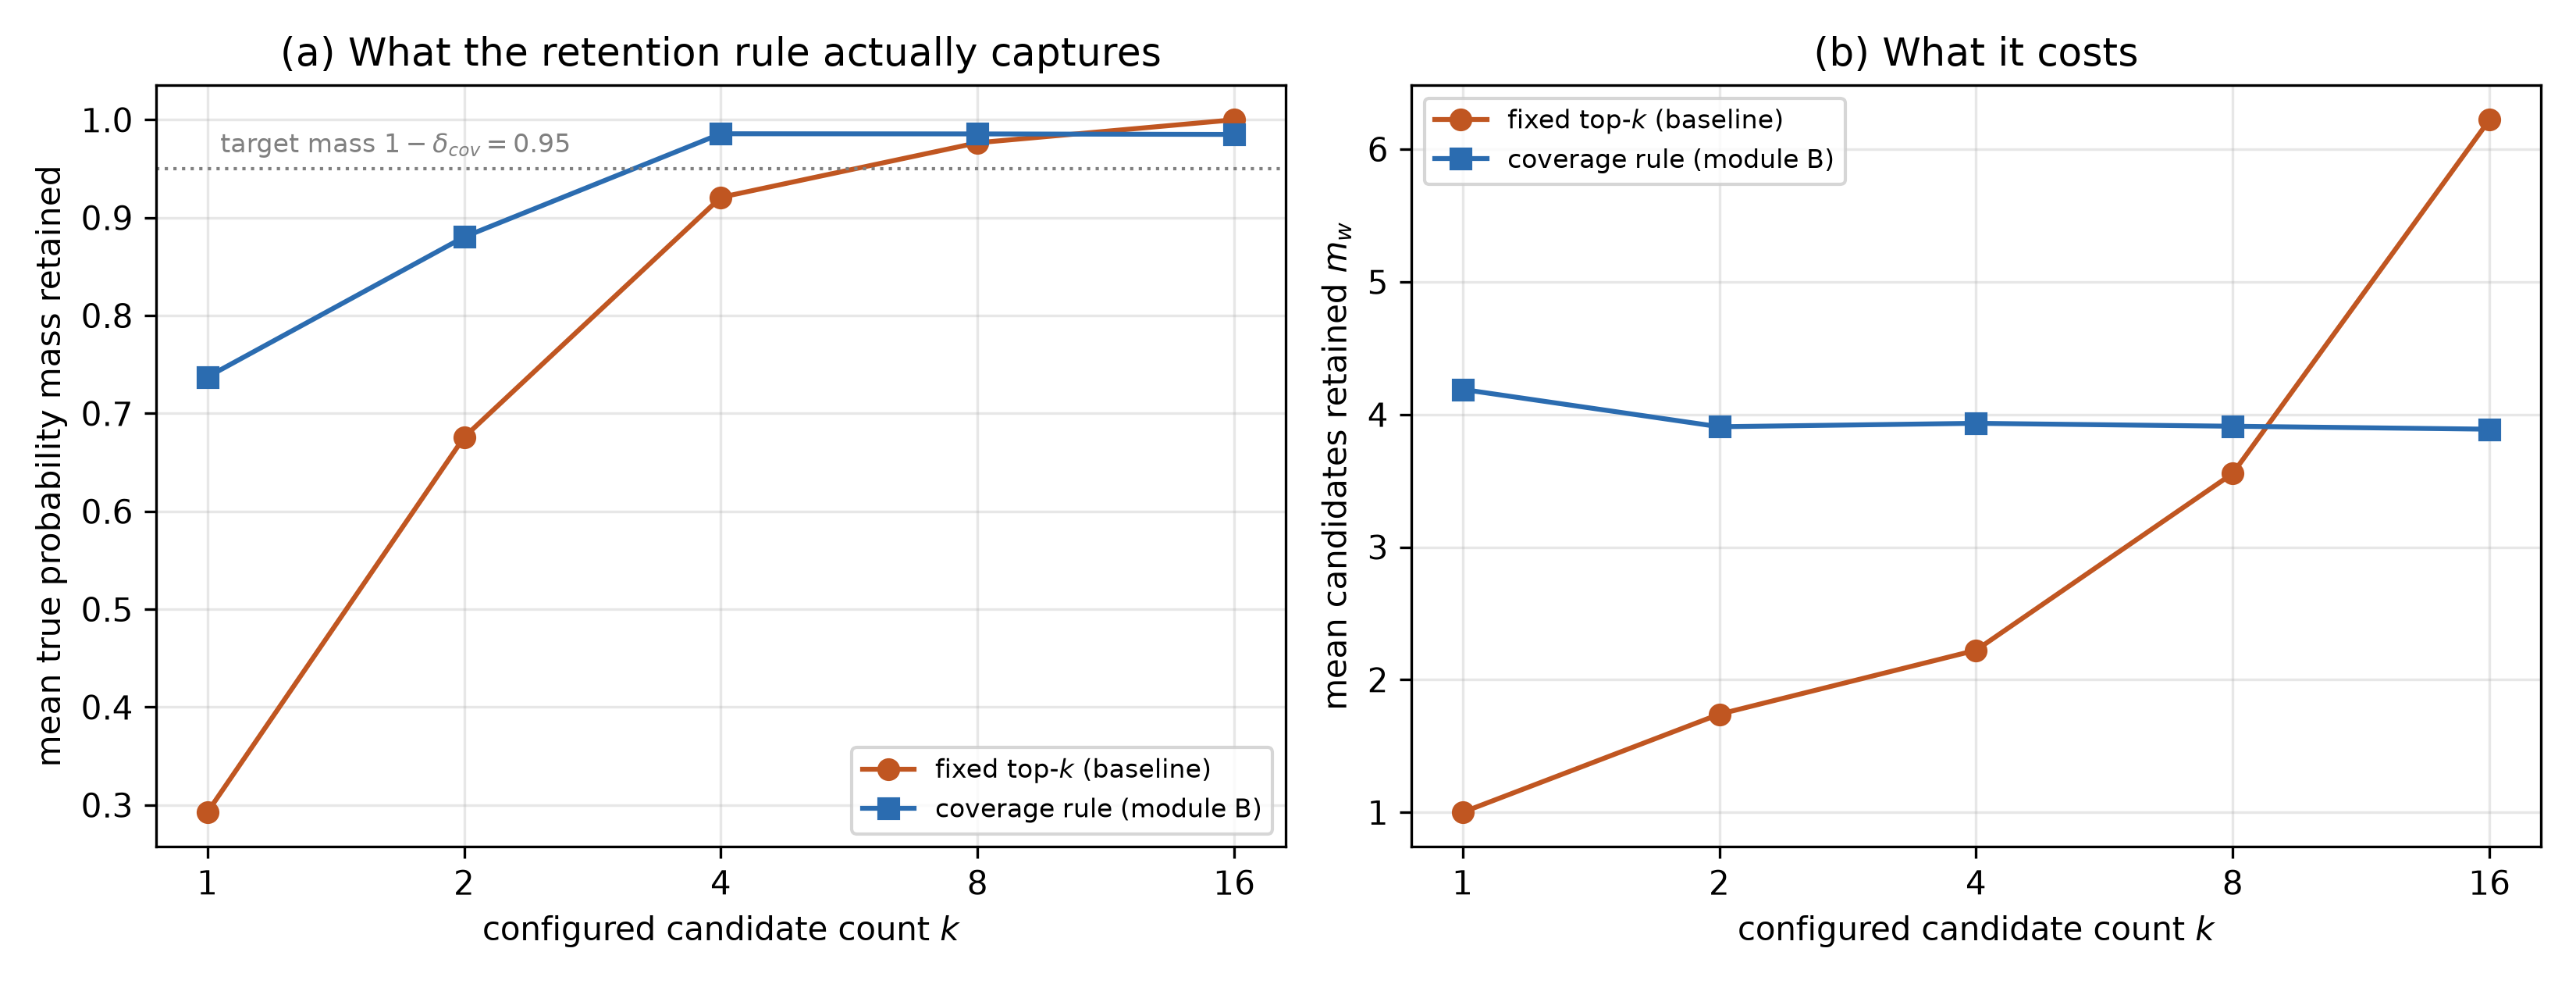
\includegraphics[width=\linewidth]{../Data/failure_study/plots/paper_figA_window_retention.png}
\caption{\textbf{Does the retention rule capture the phase information the
window carries?} \emph{(a)} Mean true probability mass retained, against the
configured candidate count $k$. Fixed top-$k$ (orange) sweeps from $0.293$
to $1.000$ across the range, so its adequacy depends entirely on $k$ being
chosen correctly; the coverage rule (blue) holds near $0.98$ from $k=4$
upward and degrades gracefully below it. The two cross at $k=16$, where the
fixed budget is generous enough to retain everything. \emph{(b)} The cost of
each, in candidates retained per window: the coverage rule is flat at
${\approx}3.9$ while the fixed rule rises linearly with $k$. Rendered from
\texttt{paperA\_window\_validation.csv}.}
\label{fig:window}
\end{figure}

\subsection{Calibration analysis: $\Cw$ ranks usefully at module D's
operating point and is not a calibrated probability estimate}
\label{sec:calibration}

Module D thresholds on $\Cw$, so it matters whether $\Cw$ means what its
scale suggests. We tested this on 2{,}687 per-window observations from
579 recaptured trials, pairing each window's predicted $\Cw$ against
ground truth: whether the observed top-1 pattern's \emph{true} noiseless
marginal really does exceed the top-2 pattern's, computed per window
specification by exact statevector simulation rather than by sampling
(\SIcalib{}).

\textbf{$\Cw$ is systematically overconfident.} The raw Brier score
\cite{brier1950} is $0.2239$, only marginally better than the $0.25$ a
constant always-0.5 forecast would achieve. In the top predicted decile
($\Cw\in(0.9,1.0]$, mean prediction $0.96$) the observed correctness rate
is $0.79$. Windows that satisfy module D's stopping rule at
$\varepsilon=0.05$ are therefore wrong roughly 21\% of the time, not 5\%.
Figure~\ref{fig:calib} shows the reliability diagrams.

\textbf{Discrimination, measured at the operating point.} Over the whole
range $\Cw$ is a modest ranking signal: its area under the ROC curve is
$0.640$ against a base rate of $0.677$. That figure averages over a range
module D never consults. D stops only when $\Cw\ge1-\varepsilon=0.95$, and
in that region the statistic is substantially more informative --- windows
above the threshold are correct $88.3\%$ of the time, against the $67.7\%$
base rate, whereas below $\Cw<0.60$ correctness falls to $54.9\%$, barely
better than a coin. Only the ordering is load-bearing for D
(Sec.~\ref{sec:moduleD}), and the ordering is real where D uses it. We
report the global AUC as well because it, not the operating-point figure,
is what bounds any \emph{other} use of $\Cw$ as a ranking signal.


This is the predicted cost of assumption (A2) being false: $b^{(1)}_w$
and $b^{(2)}_w$'s counts are negatively correlated marginals of one
Dirichlet posterior, not independent Binomials, and ignoring that
correlation pushes $\Cw$ toward more extreme values than a joint
comparison would. Isotonic regression \cite{zadrozny2002} recalibrates
the raw score to a Brier of $0.1988$ --- but that is an \emph{in-sample}
fit on the same 2{,}687 observations, with no held-out split, so it bounds
what recalibration could achieve rather than estimating out-of-sample
calibration. What it does establish is that the miscalibration has
correctable structure --- a monotone distortion, not noise --- which is
the property that makes the raw statistic usable as a ranking signal at
all. Bin-level data are in \SIcalib{}.

\textbf{We deliberately do not ship the recalibration in the default
decision rule}, and we want to be precise about why. The isotonic model
is fitted on this corpus; wiring it into module D would make the
shipped stopping rule depend on a fit whose generalisation to other
instances, orders, and window geometries we have not tested, and would
break the correspondence between the shipped configuration and the
ablation reported in the companion study~\cite{companion}, which
thresholds on raw
$\Cw$. The consequence must be stated without softening:
\textbf{$\varepsilon$ is a tuning parameter for a heuristic stopping
rule, not a statistically guaranteed error tolerance, despite its name.}

None of this contradicts module D's measured effect: a miscalibrated but
monotone statistic (Table~\ref{tab:properties}) can be a serviceable
\emph{relative} signal for ``resample this window before that one'' while
being a poor \emph{absolute} probability, and only the ordering is
load-bearing in Sec.~\ref{sec:moduleD}. Two consequences follow for an
adopter: $\varepsilon$ must be tuned empirically rather than set from a
desired error rate, and any extension consuming $\Cw$ \emph{as} a
probability --- combining it across windows, or propagating it into a
downstream posterior --- would be unsound without out-of-sample validated
recalibration, which we have not performed.

\begin{figure}[htbp]
\centering
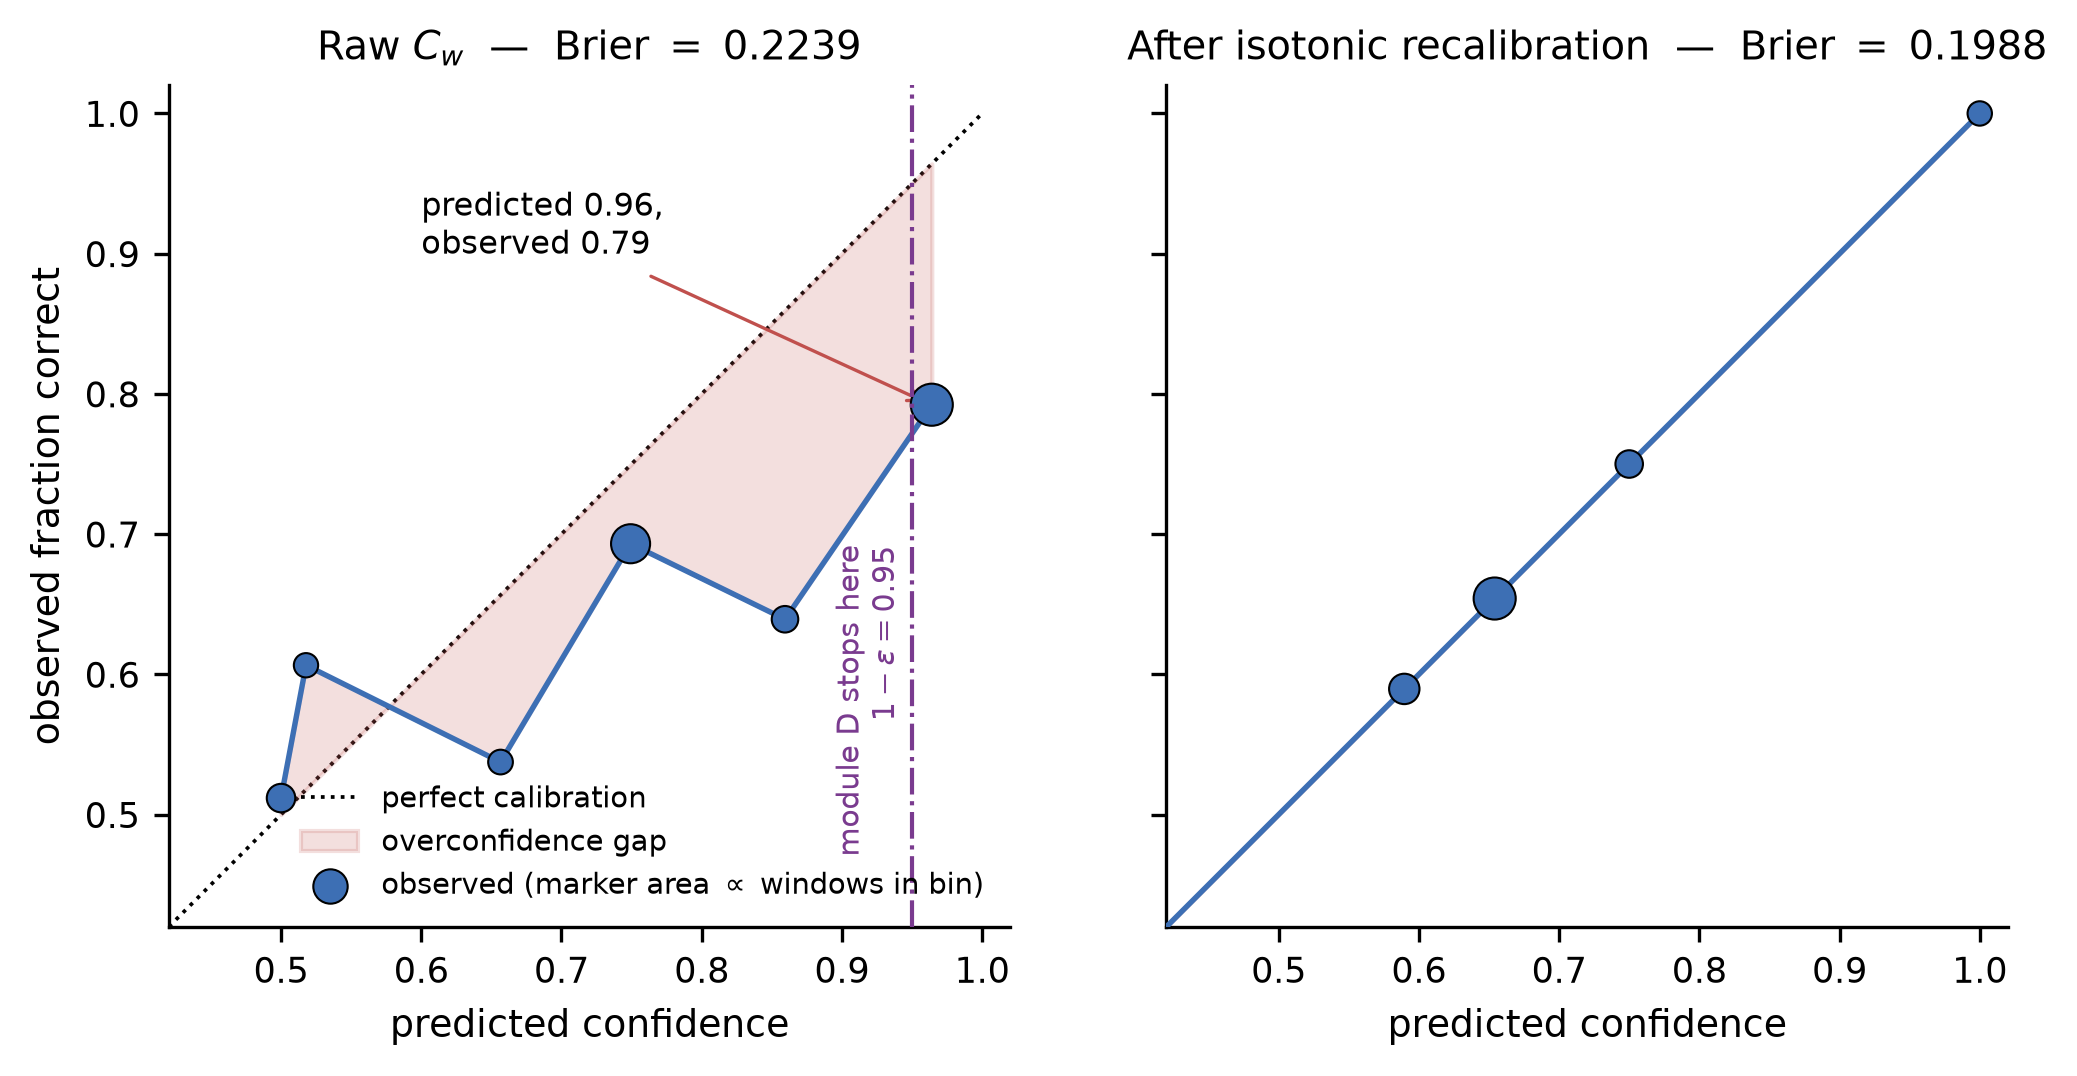
\includegraphics[width=0.94\linewidth]{../Data/failure_study/plots/paper_fig5_calibration.png}
\caption{\textbf{Does $\Cw$'s numerical value behave like a
probability?} Reliability of $\Cw$ over 2{,}687 per-window observations
from 579 trials; marker area is proportional to the number of windows in
the bin. \emph{Left:} raw $\Cw$ lies below the diagonal across the upper
range --- the shaded region is the overconfidence gap --- with Brier
$0.2239$ against $0.2500$ for a constant $0.5$ forecast. The dash-dotted
line marks module D's stopping threshold $1-\varepsilon=0.95$: windows
that halt there sit in a bin whose mean prediction is $0.96$ but whose
observed correctness is $0.79$. \emph{Right:} isotonic recalibration
reduces the Brier score to $0.1988$. \textbf{The right-hand panel is an
in-sample fit} --- isotonic regression places the bins on the diagonal by
construction --- so it establishes that the miscalibration is
\emph{correctable in principle}, not that a recalibrated $\Cw$ would
generalise. It is a diagnostic artifact and is deliberately not used by
the shipped stopping rule. Rendered from
\texttt{phase6\_calibration.csv}.}
\label{fig:calib}
\end{figure}


% =====================================================================
\section{Limitations}
\label{sec:limitations}

Four groups, ordered by how much each constrains what a reader may
conclude. Limitations bearing on the end-to-end evaluation --- external
validity of the factorisation results, and the module-by-module strength of
evidence --- belong to the companion study~\cite{companion} and are stated
there.

\paragraph{1. What the window-level result does and does not establish.}
The validation corpus is 3{,}354 windows at $N\in\{15,21\}$, noiseless and
in simulation. Two of its three instances sit at ceiling, so the reported
aggregate is carried by one instance; the corpus establishes that the
retention rule behaves as designed across a range of configured budgets,
not that it does so across a range of problem sizes. \emph{The instance
ceiling is not a choice}: the modular-arithmetic layer of our reference
implementation is a dense unitary whose compilation time rises from
$0.4$\,s at 5 work qubits to $42$\,s at 7 and exceeds a $45$\,s timeout at
8. \emph{The noiseless scope is a choice}, made to isolate the mechanism.
Modules B and C act only on already-sampled counts, but module D is more
exposed: under a noise floor, additional shots can sharpen confidence in a
wrong pattern while consuming the $\Smax$ budget. We make no claim about
behaviour under noise in either direction. \emph{Closing these:} a
reversible modular-arithmetic circuit \cite{cuccaro2004} for the ceiling;
re-running the released grid with the noise models already in the code.

\paragraph{2. The gain is budget selection, not placement.}
Against controls given each module's own realised budget to spend
uniformly, no individual module is distinguishable from its control; the
analysis is in the companion study~\cite{companion} and the conclusion
constrains this article directly. We therefore do not claim that per-window
placement is intrinsically better than an equal allocation of the same
resources. The supported claim is narrower and is the one made throughout:
the rule recovers a workable budget from the measured counts without being
given one. The window-level result of Sec.~\ref{sec:wresults} is consistent
with exactly that reading --- module B is marginally worse than the best
fixed budget and far better than a poorly chosen one.

\paragraph{3. The confidence model.}
$\Cw$'s independence assumption (A2) is measurably false, and the
calibration study quantifies the cost: raw Brier $0.2239$ against $0.2500$
for a constant $0.5$ forecast, with the top predicted bin at $0.96$
predicted against $0.79$ observed, and a global AUC of $0.640$. The
consequence is that $\varepsilon$ names an error target but delivers a
heuristic threshold on an uncalibrated statistic; it must be tuned
empirically rather than set from a desired error rate, and any extension
consuming $\Cw$ as a probability --- combining it across windows, or
propagating it into a downstream posterior --- would be unsound. The
isotonic recalibration is deliberately not wired into the shipped rule, so
that the shipped configuration is the one that was evaluated --- and in any
case it was fitted and evaluated in-sample on the same 2{,}687
observations, so its $0.1988$ bounds what recalibration could achieve
rather than estimating out-of-sample performance. Separately, $\Cw$
compares only the top two patterns (A3), so a genuine three-way near-tie is
not flagged as low-confidence: a structural blind spot rather than a tuned
trade-off, accepted given $\ell_w\le6$ throughout our corpus.
\emph{Closing these:} a Dirichlet-joint formulation of
Eq.~\eqref{eq:cw}; a held-out calibration split.

\paragraph{4. Parameters, coverage, and deliberate scope exclusions.}
$\varepsilon$ and $\dcov$ were used at their defaults
(Sec.~\ref{sec:parameters}) because those defaults already produced large
effects, so no calibration failure prompted a search; we do not know how
sensitive the reported effects are to them. \textbf{Module B carries no
population coverage guarantee}: $\dcov$ bounds coverage of the observed
sample, not the probability that the true pattern is retained, and
Sec.~\ref{sec:wresults} measures the resulting shortfall at 59\% of
windows. Closing that requires a finite-sample concentration bound we
neither derive nor implement. Window geometry is fixed at configuration
time and never revised in response to confidence (A5), so the ambiguity
boundary failure mode --- within ${\sim}1\%$ of a window's $0.5$ boundary
the winning bucket is unstable across repeated identical measurements ---
is untouched by this framework, which by construction cannot revise
geometry without regenerating circuits. Each window is also allocated
independently, with no shared budget across windows (A4).

% =====================================================================
\section*{Ethics statements}
This work involved no human participants, no animal subjects, and no data
collected from social media platforms. All data are generated by
numerical simulation.

\section*{CRediT author statement}
\noindent
Sanjay Lakshmanan R: Conceptualization, Methodology, Software,
Validation, Formal analysis, Investigation, Data curation,
Writing -- original draft, Writing -- review \& editing, Visualization.

\section*{Declaration of competing interest}
The author declares no known competing financial interests or personal
relationships that could have appeared to influence the work reported in
this paper.

\section*{Relation to the companion article}
The method specified here is evaluated end to end in a companion
study~\cite{companion}, which reports the failure-mode characterisation
that motivated it, the five-arm ablation, generalisation to pre-registered
held-out instances, and the matched-resource controls that qualify the
result. The two articles share one released corpus and one code archive,
and analyse it at different units: this article at the window, the
companion at the trial. No figure, table, or result is common to both.

\section*{Reproducibility}

Every numeric claim in this article is a mechanical summary of a released
result file; \SIartifacts{} maps each file to the script that produced it
and the section that consumes it.

\textbf{Trials are deterministic given their seed.} Each trial's seed is
derived from its grid coordinates and seeds Aer's sampling, so re-running
any cell reproduces its counts exactly. This was verified rather than
assumed: an instrumented re-run reproduced all 144 canonical trials, in all
five arms, bit-for-bit.

\textbf{The window-level analysis recomputes nothing.} The retention script
replays frozen per-window counts through the shipped candidate-generation
functions and scores them against statevector marginals; it samples no
circuit and asserts the reported calibration figures before writing.

\textbf{Long runs are resumable.} A completed trial is skipped on restart by
its seed, so an interrupted campaign resumes without altering any result.

\section*{Code availability}
The complete implementation --- quantum circuits, classical reconstruction,
the adaptive modules, and every experiment script named in \SIartifacts{}
--- is released under the Apache-2.0 licence at
\url{https://github.com/Shadow-46/QuantumPhaseReconstruction}. An archived
snapshot will be deposited in a persistent repository and its DOI supplied
at acceptance. The modules described in this article are implemented in
\texttt{Reconstruction/\allowbreak{}confidence.py} (the statistic $\Cw$),
\texttt{Reconstruction/\allowbreak{}candidate\_\allowbreak{}generation.py}
(module B), and
\texttt{Algorithms/\allowbreak{}adaptive\_\allowbreak{}reconstruction.py}
(modules C and D, and the switchable reconstruction path of
Invariant~\ref{prop:baseline}). Module D deliberately sits above
\texttt{Reconstruction/}, which imports nothing from the circuit layer, for
the reason given in step 3 of Sec.~\ref{sec:protocol}. Each executable
module carries a self-test that runs without arguments.

\section*{Data availability}
All raw per-trial records, per-window recaptured counts, summary tables,
and figures are released with the code at the same location. No data were
obtained from third parties, and no dataset is under embargo.

\section*{Supplementary material}
A Supplementary Information document accompanies this article, containing
the complete derivations of the properties summarised in
Table~\ref{tab:properties} and the bin-level calibration data. It is not
required to understand the method or to judge the central claims; it is
what allows them to be verified independently.

% =====================================================================
\bibliographystyle{elsarticle-num}
\bibliography{refs_A}

\end{document}
